\section{Implementation Details}
\label{sec:implementation}
The code and additional results are publicly available at \url{https://github.com/junyanz/BicycleGAN}. Please refer to our website for more details about the datasets, architectures, and training procedures.
\begin{figure}
\centering
% \hspace{-.08\linewidth}
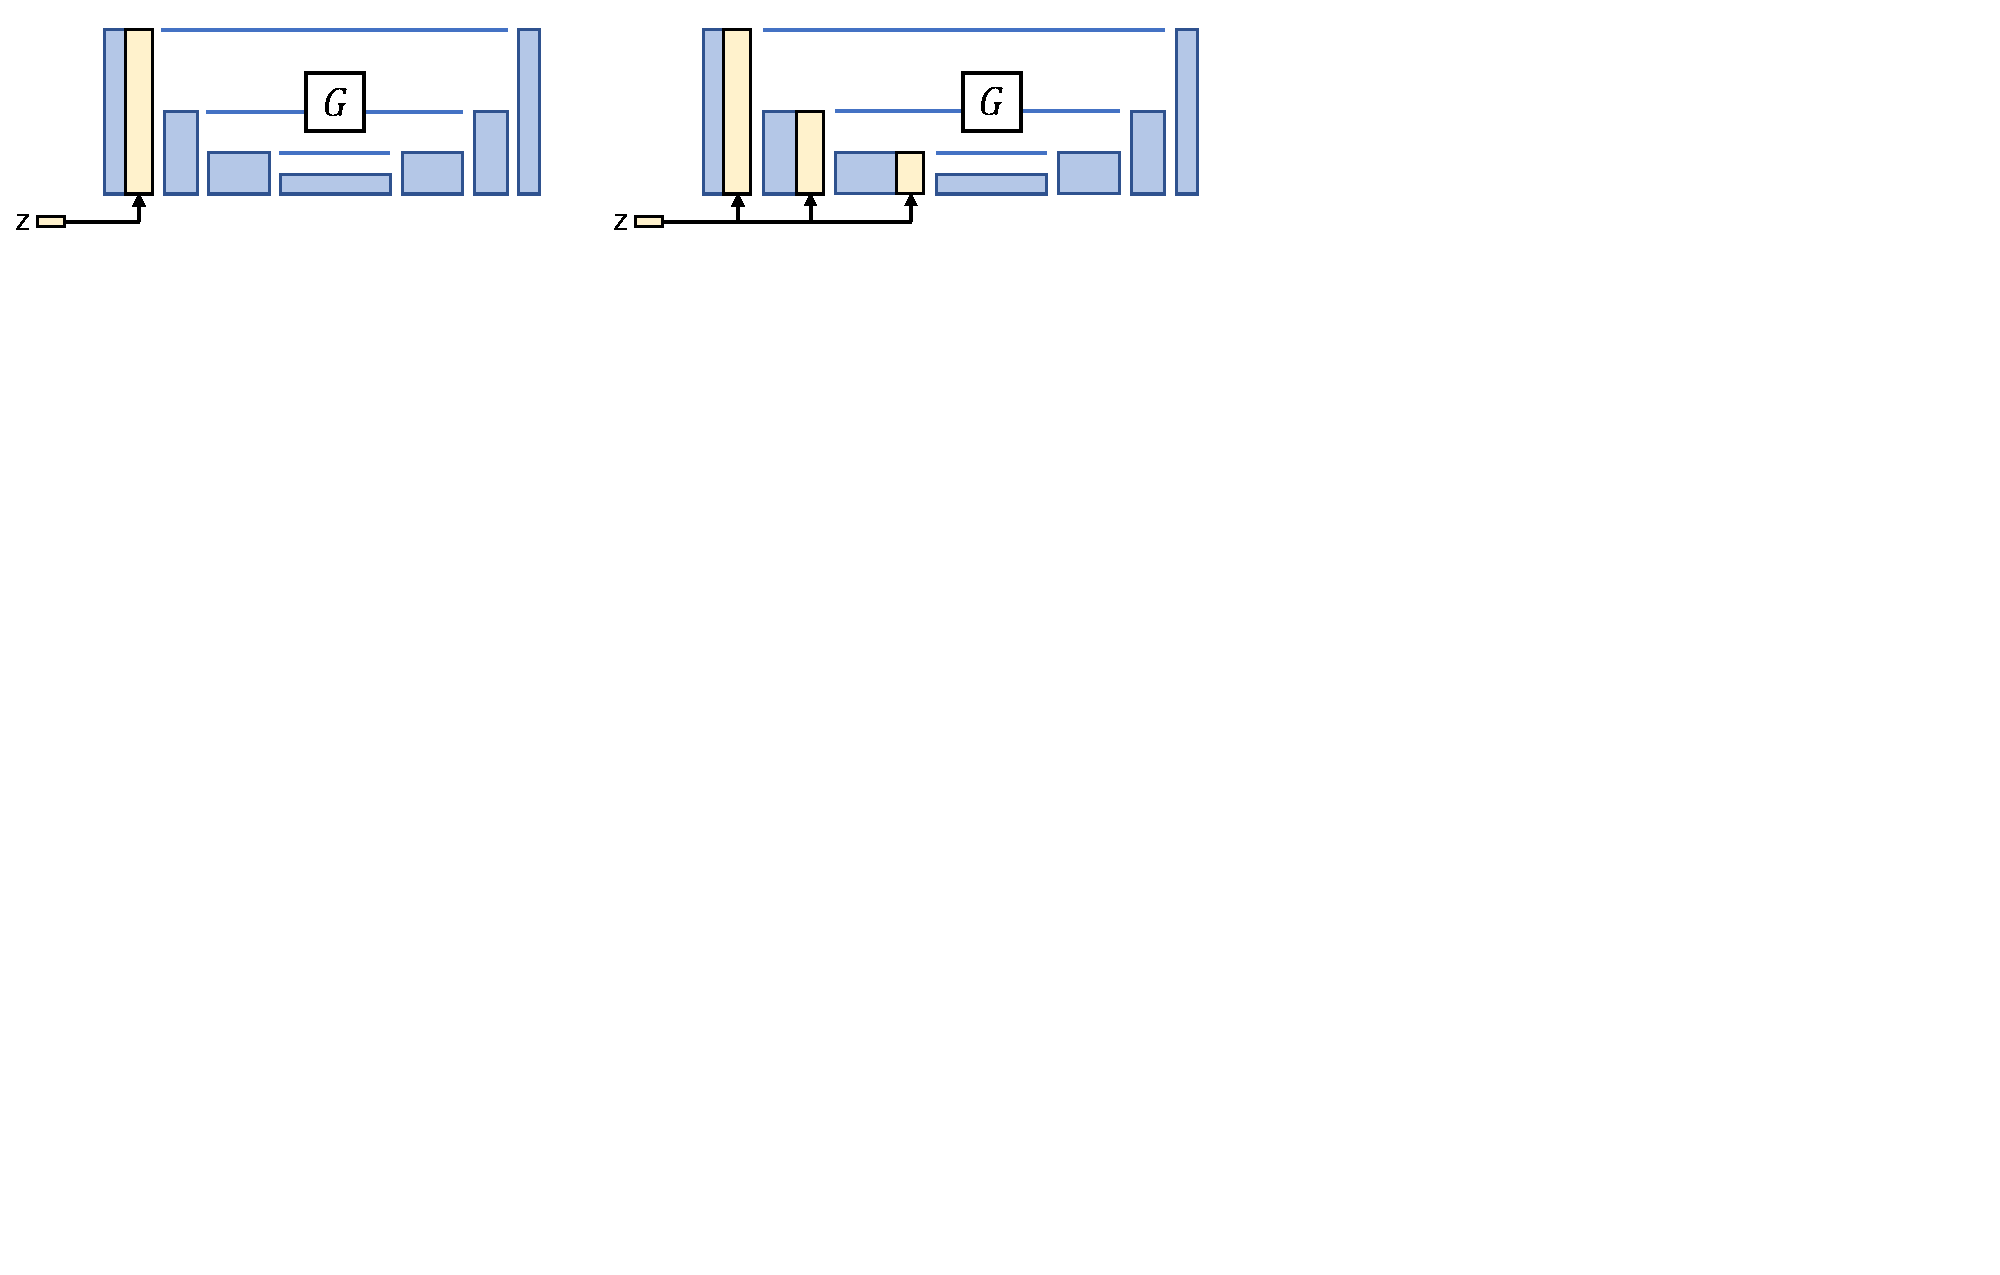
\includegraphics[width=1.0\linewidth]{imgs/injectz.pdf}
\caption{\small \textbf{Alternatives for injecting {\bf z} into generator.} Latent code \textbf{z} is injected by spatial replication and concatenation into the generator network. We tried two alternatives, {\bf (left)} injecting into the input layer and {\bf (right)} every intermediate layer in the encoder.}
\vspace{-4mm}
\label{fig:addz}
\end{figure}

\paragraph{Network architecture} For generator $\G$, we use the U-Net~\citep{ronneberger2015u}, which contains an encoder-decoder architecture, with symmetric skip connections. The architecture has been shown to produce strong results in the unimodal image prediction setting when there is a spatial correspondence between input and output pairs. For discriminator $\D$, we use two PatchGAN discriminators~\citep{isola2016image} at different scales, which aims to predict real vs. fake for $70\times 70$ and $140 \times 140$ overlapping image patches. For the encoder $\E$, we experiment with two networks: (1) \texttt{E\textsubscript{CNN}}: CNN with a few convolutional and downsampling layers and (2) \texttt{E\textsubscript{ResNet}}: a classifier with several residual blocks~\cite{he2016deep}.

\paragraph{Training details} We build our model on the Least Squares GANs (LSGANs) variant~\citep{mao2016least}, which uses a least-squares objective instead of a cross entropy loss. LSGANs produce high-quality results with stable training. We also find that not conditioning the discriminator $\D$ on input $\mathbf{A}$ leads to better results (also discussed in~\citep{pathakCVPR16context}), and hence choose to do the same for all methods. We set the parameters $\lambda_{\text{image}}=10$, $\lambda_{\text{latent}}=0.5$ and $\lambda_{\text{KL}}=0.01$ in all our experiments. We tie the weights for the generators and encoders in the \cvaegan and \cinfogan models. For the encoder, only the predicted mean is used in \cinfogan. We observe that using two separate discriminators yields slightly better visual results compared to sharing weights. We only update $\G$ for the $\ell_1$ loss $\mathcal{L}_{1}^{\text{latent}}(\G,\E)$ on the latent code (Equation \ref{eqn:L1_lacyc}), while keeping $\E$ fixed. We found optimizing $\G$ and $\E$ simultaneously for the loss would encourage $G$ and $E$ to hide the information of the latent code without learning meaningful modes.
We train our networks from scratch using Adam~\citep{kingma2014adam} with a batch size of $1$ and with a learning rate of $0.0002$. We choose latent dimension $|\z|=8$ across all the datasets. 

{\bf Injecting the latent code $\z$ to generator}.
We explore two ways of propagating the latent code $\z$ to the output, as shown in Figure~\ref{fig:addz}: 
(1) \texttt{add\_to\_input}: we spatially replicate a $Z$-dimensional latent code $\z$ to an $H\!\times W\!\times Z$ tensor and concatenate it with the $H\!\times W\!\times 3$ input image and (2)~\texttt{add\_to\_all}: we add $\z$ to each intermediate layer of the network $\G$, after spatial replication to the appropriate sizes.

\vspace{-1mm}